%%%%%%%%%%%%%%%%%%%%%%%%
%
% $Autor: Hemanth Jadiswami Prabhakaran $
% $Datum: 2026-09-12 $
% $Pfad: GitHub/MBIDA_Thesis/report/Contents/General/en/03DomainMachineLearning.tex $
% $Version: 1 $
%
% $Project: MBIDA Thesis $
%
%%%%%%%%%%%%%%%%%%%%%%%%

\chapter{Domain Machine Learning}
\label{chap:domainML}

This chapter introduces the forecasting methods compared in this thesis: three base forecasting models used to produce an initial, independent prediction for every series in the hierarchy, and three reconciliation methods used to make those independent predictions consistent with one another across the hierarchy. Section~\ref{sec:baseModels} covers the base models, and Section~\ref{sec:hierarchicalCoherence} introduces the concept of hierarchical coherence and the summing matrix that formalises it. Section~\ref{sec:reconciliationTheory} then presents the three reconciliation strategies built on that formalism. The specific configuration of these methods for the M5 dataset -- the hierarchy levels used, the seasonal period, and the particular MinTrace variant applied -- is a design decision covered in Chapter~\ref{chap:methodology}, and their implementation is described in Chapter~\ref{chap:appDevelopment}. Empirical results comparing all combinations of base model and reconciliation method appear in Chapter~\ref{chap:evaluation}.

\section{Base Forecasting Models}
\label{sec:baseModels}

Three base forecasting models are used in this thesis, chosen to span a deliberately narrow range of sophistication: a naive reference model, a classical exponential smoothing method, and a decomposition-based method with a strong track record in forecasting competitions. Each model is fitted independently to every series in the hierarchy -- from the single Total series down to each individual item-store combination -- with no awareness of the hierarchical structure the series sit within. It is this independence that creates the coherence problem addressed in Section~\ref{sec:hierarchicalCoherence}.

\subsection{HistoricAverage}
\label{subsec:histAvg}

The simplest of the three models, HistoricAverage, forecasts every future period as the arithmetic mean of all previously observed values of the series -- the "average method" in the standard taxonomy of simple forecasting benchmarks \cite{Hyndman:2018}:
\[
\hat{y}_{t+h} = \frac{1}{T}\sum_{i=1}^{T} y_i, \qquad \text{for every horizon } h.
\]
It has no concept of trend or seasonality, and its forecast is flat across the entire horizon. Despite its simplicity, HistoricAverage serves a specific methodological purpose in this thesis beyond being a discardable baseline: because it is a linear function of the training data, it is already perfectly coherent across a hierarchy without any reconciliation step being applied, since the mean of a sum of series equals the sum of their individual means. This property makes it a natural sanity check for the reconciliation pipeline itself, and it also functions as the fallback model whenever the more sophisticated models below fail to fit a particular series (Chapter~\ref{chap:appDevelopment}).

\subsection{Exponential Smoothing (ETS)}
\label{subsec:ets}

Exponential smoothing methods forecast a series by taking a weighted average of past observations, with the weights decaying exponentially the further back in time an observation lies. In its simplest form, this is written recursively as
\[
\hat{y}_{t+1} = \alpha y_t + (1-\alpha) \hat{y}_t , \qquad 0 \le \alpha \le 1,
\]
so that each new forecast blends the latest observation with the previous forecast, and the smoothing parameter $\alpha$ controls how quickly the influence of older observations decays. The ETS (Error, Trend, Seasonal) framework formalises this idea as a state-space model in which each of the three components -- the error structure, the trend, and the seasonal pattern -- can independently be absent, additive, or multiplicative \cite{Hyndman:2008}. Rather than requiring the analyst to specify which combination of components applies to a given series, an automated ETS procedure fits every valid combination and selects the one that best balances fit and parsimony according to an information criterion. This automatic model selection is what makes ETS practical to apply, unmodified, across tens of thousands of series with very different characteristics, as is required in Chapter~\ref{chap:appDevelopment}. Where a seasonal component is included, the model requires a seasonal period to be specified; the rationale for the specific period used in this thesis is given in Chapter~\ref{chap:methodology}.

\subsection{The Theta Method}
\label{subsec:theta}

The Theta method decomposes a series into two or more "theta lines" -- transformed versions of the original series in which the local curvature (the second difference) is scaled by a coefficient $\theta$. Formally, a theta line $Z_t(\theta)$ is defined as the series whose second differences are a scaled version of the original series' own:
\[
\nabla^2 Z_t(\theta) = \theta\, \nabla^2 y_t ,
\]
where $\nabla^2$ denotes the second-difference operator and $y_t$ is the original series \cite{Assimakopoulos:2000}. A $\theta$ value below one dampens short-term fluctuations, producing a smoother, longer-term view of the series' level, while a $\theta$ value above one amplifies them, emphasising short-term dynamics. The classical implementation combines a long-term line ($\theta = 0$, equivalent to a linear trend) with a short-term line ($\theta = 2$) in equal weight, after first removing any seasonal component so that the decomposition operates on a deseasonalised series \cite{Assimakopoulos:2000}. The method was the strongest performer in the M3 forecasting competition, and its combination of a simple decomposition step with strong empirical accuracy is the reason it is included here as the most sophisticated of the three base models.

\section{Hierarchical Coherence and the Summing Matrix}
\label{sec:hierarchicalCoherence}

A hierarchical time series structure arranges a collection of series so that some are the sum of others: a company total is the sum of its regions, each region is the sum of its stores, and so on down to the most granular, or \emph{bottom-level}, series that are not themselves the sum of anything else in the structure. When every node in the structure belongs to exactly one parent, the result is a \emph{simple tree} hierarchy; structures in which a series can be classified along more than one dimension at once (for example, jointly by region and by product brand) instead form \emph{grouped} or \emph{cross-product} hierarchies, which require a different aggregation treatment \cite{Hyndman:2018}. This distinction, and which of the two applies to the dataset used in this thesis, is addressed in Chapter~\ref{chap:methodology}.

Forecasting every series in such a structure independently -- fitting a separate model to the company total and a separate model to each individual store, with no link between the two -- produces forecasts that are individually reasonable but collectively \emph{incoherent}: there is no guarantee that the sum of the store-level forecasts will equal the independently produced total-level forecast. Hierarchical forecasting formalises the relationship between levels using a \emph{summing matrix}, conventionally denoted $S$, which encodes exactly how each bottom-level series contributes to every aggregate series above it. If $b_t$ denotes the vector of bottom-level values at time $t$, the complete set of values across every level of the hierarchy, $y_t$, is given by
\[
y_t = S\, b_t .
\]
A set of forecasts is coherent precisely when it also satisfies this relationship: the forecasts at every aggregate level must be recoverable from the bottom-level forecasts via the same matrix $S$ that defines how the actual data aggregates \cite{Hyndman:2018}. Since independently fitted base forecasts generally do not satisfy this relationship, a subsequent \emph{reconciliation} step is required to enforce it.

Every reconciliation method considered in this thesis can be written as a single general transformation of the base forecasts:
\[
\tilde{y}_t = S\, G\, \hat{y}_t ,
\]
where $\hat{y}_t$ is the vector of independently produced base forecasts across \emph{every} level of the hierarchy, $G$ is a matrix that maps this full, generally incoherent set of base forecasts onto a single reconciled estimate of the bottom level, and post-multiplying by $S$ re-aggregates that reconciled bottom level back up through every level above it -- guaranteeing coherence by construction, whatever $G$ turns out to be \cite{Wickramasuriya:2019}. The three reconciliation strategies compared in this thesis differ only in how $G$ is constructed; each is presented next as a specific, named choice of this one matrix.

\section{Reconciliation Theory}
\label{sec:reconciliationTheory}

Reconciliation methods differ in how much they trust the base forecast produced at each level of the hierarchy, ranging from complete trust in the bottom level, to complete trust in the top level, to a compromise that adjusts every level simultaneously. Figure~\ref{fig:reconciliationFlow} contrasts the three methods by the direction information flows between levels: strictly upward for Bottom-Up, strictly downward for Top-Down, and simultaneously in both directions for MinT.

\begin{figure}[H]
	\centering
	\resizebox{\textwidth}{!}{% Information-flow direction under Bottom-Up, Top-Down, and MinT reconciliation
% Panels stacked vertically, scaled down proportionally using scale and transform shape.
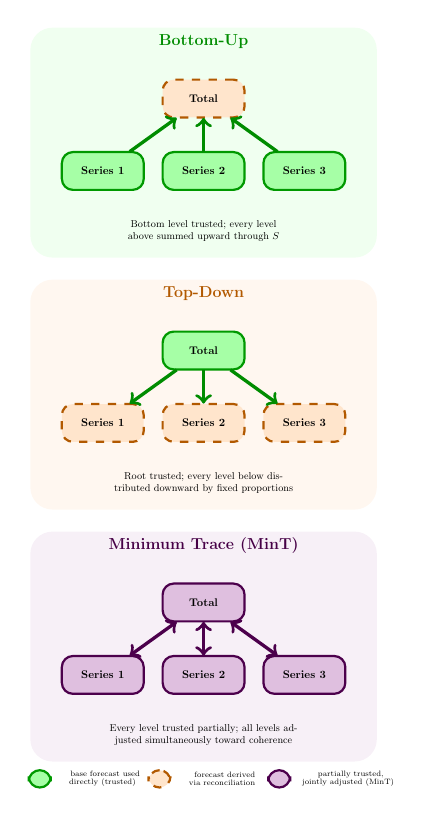
\begin{tikzpicture}[
	scale=0.4,
	every node/.style={transform shape},
	node distance   = 1.4cm and 1cm,
	topstage/.style   = {rectangle, rounded corners, thick, minimum width=2.6cm,
		minimum height=1.2cm, align=center, font=\normalsize\bfseries},
	leafstage/.style  = {rectangle, rounded corners, thick, minimum width=2.6cm,
		minimum height=1.2cm, align=center, font=\normalsize\bfseries},
	trusted/.style    = {fill=green!35, draw=green!60!black},
	derived/.style    = {fill=orange!20, draw=orange!70!black, dashed},
	minttrust/.style  = {fill=violet!25, draw=violet!60!black},
	title/.style      = {font=\Large\bfseries},
	detail/.style     = {align=center, font=\small, text width=9.5cm},
	legendbox/.style  = {rectangle, rounded corners, thick, minimum width=0.7cm, minimum height=0.55cm},
	panelbg/.style    = {rectangle, rounded corners=8pt, draw=none, minimum width=11cm, minimum height=7.3cm}
	]
	
	% ===================== Panel 1: Bottom-Up =====================
	\begin{scope}[yshift=0cm]
		\node[panelbg, fill=green!6] at (0,0.9) {};
		\node[title, color=green!55!black] (t1) at (0, 4.1) {Bottom-Up};
		
		\node[topstage, derived]  (tot1) at (0, 2.3)   {Total};
		\node[leafstage, trusted] (b1a)  at (-3.2, 0) {Series 1};
		\node[leafstage, trusted] (b1b)  at (0, 0)    {Series 2};
		\node[leafstage, trusted] (b1c)  at (3.2, 0)  {Series 3};
		
		\draw[->, very thick, green!55!black] (b1a) -- (tot1);
		\draw[->, very thick, green!55!black] (b1b) -- (tot1);
		\draw[->, very thick, green!55!black] (b1c) -- (tot1);
		
		\node[detail] at (0, -1.9) {Bottom level trusted; every level above summed upward through $S$};
	\end{scope}
	
	% ===================== Panel 2: Top-Down =====================
	\begin{scope}[yshift=-8cm]
		\node[panelbg, fill=orange!6] at (0,0.9) {};
		\node[title, color=orange!70!black] (t2) at (0, 4.1) {Top-Down};
		
		\node[topstage, trusted]  (tot2) at (0, 2.3)   {Total};
		\node[leafstage, derived] (b2a)  at (-3.2, 0) {Series 1};
		\node[leafstage, derived] (b2b)  at (0, 0)    {Series 2};
		\node[leafstage, derived] (b2c)  at (3.2, 0)  {Series 3};
		
		\draw[->, very thick, green!55!black] (tot2) -- (b2a);
		\draw[->, very thick, green!55!black] (tot2) -- (b2b);
		\draw[->, very thick, green!55!black] (tot2) -- (b2c);
		
		\node[detail] at (0, -1.9) {Root trusted; every level below distributed downward by fixed proportions};
	\end{scope}
	
	% ===================== Panel 3: MinT =====================
	\begin{scope}[yshift=-16cm]
		\node[panelbg, fill=violet!6] at (0,0.9) {};
		\node[title, color=violet!55!black] (t3) at (0, 4.1) {Minimum Trace (MinT)};
		
		\node[topstage, minttrust]  (tot3) at (0, 2.3)   {Total};
		\node[leafstage, minttrust] (b3a)  at (-3.2, 0) {Series 1};
		\node[leafstage, minttrust] (b3b)  at (0, 0)    {Series 2};
		\node[leafstage, minttrust] (b3c)  at (3.2, 0)  {Series 3};
		
		\draw[<->, very thick, violet!60!black] (b3a) -- (tot3);
		\draw[<->, very thick, violet!60!black] (b3b) -- (tot3);
		\draw[<->, very thick, violet!60!black] (b3c) -- (tot3);
		
		\node[detail] at (0, -1.9) {Every level trusted partially; all levels adjusted simultaneously toward coherence};
	\end{scope}
	
	% ===================== Shared legend =====================
	\begin{scope}[yshift=-19.3cm]
		\node[legendbox, trusted] (legA) at (-5.2, 0) {};
		\node[detail, text width=3cm, anchor=west, font=\scriptsize] at (legA.east) {\; base forecast used directly (trusted)};
		
		\node[legendbox, derived] (legB) at (-1.4, 0) {};
		\node[detail, text width=3cm, anchor=west, font=\scriptsize] at (legB.east) {\; forecast derived via reconciliation};
		
		\node[legendbox, minttrust] (legC) at (2.4, 0) {};
		\node[detail, text width=3.4cm, anchor=west, font=\scriptsize] at (legC.east) {\; partially trusted, jointly adjusted (MinT)};
	\end{scope}
	
\end{tikzpicture}}
	\caption{Information flow between hierarchy levels under each reconciliation strategy.}\label{fig:reconciliationFlow}
\end{figure}

\subsection{Bottom-Up}
\label{subsec:bottomUp}

The Bottom-Up approach forecasts only the bottom-level series directly, and obtains every aggregate-level forecast by summing the relevant bottom-level forecasts through the summing matrix $S$ \cite{Orcutt:1968, Dunn:1976}. In terms of the general reconciliation matrix $G$ introduced in Section~\ref{sec:hierarchicalCoherence}, this is the simplest possible choice available: $G = [\, \mathbf{0} \mid I \,]$, a matrix that discards every base forecast produced at an aggregate level entirely and passes the bottom-level base forecasts through completely unchanged. Because it relies exclusively on the most disaggregated forecasts, Bottom-Up preserves all information available at the item level and never overrides it with a top-down assumption. The trade-off is that bottom-level series are typically the noisiest and, in a retail setting, the most intermittent in the hierarchy, so any forecasting error made at that level propagates directly, and without correction, into every aggregate forecast above it.

\subsection{Top-Down}
\label{subsec:topDown}

The Top-Down approach forecasts only the single series at the root of the hierarchy, and distributes that top-level forecast downward to every lower level using a set of disaggregation proportions, most commonly each series' historical average share of the total \cite{Gross:1990}. In terms of the same general matrix $G$, this corresponds to a matrix with a single non-zero column -- the one selecting the top-level base forecast -- populated with the disaggregation proportions $p$: every reconciled bottom-level estimate is simply a fixed share of that one top-level number, and every other base forecast produced anywhere else in the hierarchy is discarded. Because the root-level series is typically the most stable and least intermittent series in the entire hierarchy, its forecast is comparatively easy to produce accurately. The trade-off runs in the opposite direction to Bottom-Up: Top-Down cannot represent a lower-level series' own trend or seasonal pattern if that pattern differs from its historical share of the total, which can introduce systematic bias at the lower levels of the hierarchy \cite{Wickramasuriya:2019}. Top-Down reconciliation is only well defined when the hierarchy has a single root series to distribute downward from; how this condition is ensured for the dataset used in this thesis is addressed in Chapter~\ref{chap:methodology}.

\subsection{Minimum Trace (MinT)}
\label{subsec:minTrace}

Rather than committing entirely to the bottom level or the top level, the Minimum Trace (MinT) framework adjusts the base forecasts at every level of the hierarchy simultaneously, choosing the $G$ matrix that minimises the total variance of the reconciled forecast errors, subject to the requirement that the result remains coherent under $S$ \cite{Wickramasuriya:2019}. Formally, this optimal $G$ has the closed form
\[
G = \left( S^{\top} W^{-1} S \right)^{-1} S^{\top} W^{-1} ,
\]
where $W$ is the covariance matrix of the base forecasts' errors \cite{Wickramasuriya:2019}. This is a generalised least-squares projection of the base forecasts onto the coherent subspace defined by $S$, weighted by exactly how much each series' base forecast can be trusted relative to the others. The original formulation allows this covariance estimate $W$ to range from a simple structural approximation,
\[
W = \operatorname{diag}(S \mathbf{1}) ,
\]
where $\mathbf{1}$ is a vector of ones -- so that each node's weight is simply the count of bottom-level series summing into it, the row sums of $S$ itself -- to a full shrinkage estimator of the sample error covariance \cite{Wickramasuriya:2019}. At the scale of a large retail hierarchy with tens of thousands of bottom-level series, estimating a full covariance matrix becomes computationally prohibitive, which is why implementations of MinT commonly offer a structurally-scaled variant as a tractable approximation; the specific variant used in this thesis, and the trade-off this choice implies, is discussed in Chapter~\ref{chap:methodology}.

MinT is generally presented in the literature as the theoretically preferred reconciliation method, since Bottom-Up and Top-Down can each be shown to be special, restrictive cases of the same $G$ framework introduced above \cite{Wickramasuriya:2019}: both are recoverable as particular, fixed choices of $G$, while MinT is the specific choice proven to be optimal. This generalised least-squares approach to reconciliation predates MinT itself, however: reconciling every level of a hierarchy simultaneously through a regression-style combination of the independently produced base forecasts was first shown to improve on both Bottom-Up and Top-Down at once, using a simple weighting scheme based only on the hierarchy's structure \cite{Hyndman:2011}. What Wickramasuriya et al. added, and what the "Min" in MinT's name refers to, is the proof that setting $W$ to the true covariance of the base forecast errors minimises the trace of the reconciled error covariance among all reconciliations that preserve unbiasedness ($SGS = S$), provided the base forecasts are themselves unbiased \cite{Wickramasuriya:2019}. Top-Down lies outside this class, and clipped base forecasts are no longer strictly unbiased. Because the true covariance is unknown, every practical MinT variant approximates it: the structural scaling $W = \operatorname{diag}(S\mathbf{1})$, introduced by \textcite{Athanasopoulos:2017}, is the simplest such approximation rather than the optimal weighting itself, and the non-negativity constraint used in this thesis follows \textcite{Wickramasuriya:2020}.

Whether this theoretical advantage is realised in practice depends on how well the chosen covariance approximation reflects the true error structure of the series being reconciled -- a question this thesis investigates empirically in Chapter~\ref{chap:evaluation}.